\documentclass{article}

\usepackage{graphicx}
\usepackage{subfigure}

\usepackage{tikz}
\usetikzlibrary{positioning}

\begin{document}

\begin{figure}
  \subfigure[Antes da rotação]{
    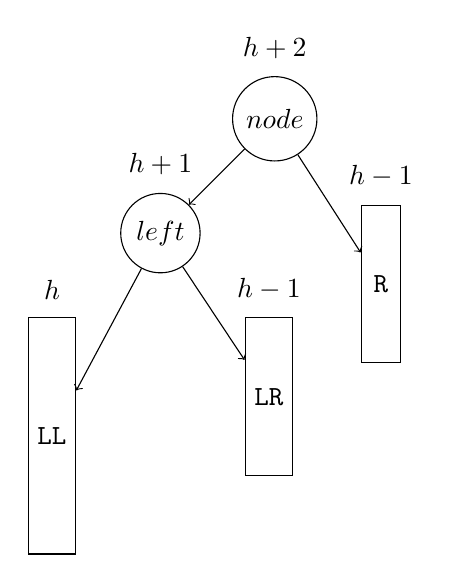
\begin{tikzpicture}
      \node[circle, draw] (node) at (1, 1) {$node$};
      \node[circle, draw] (left) [below left = 1cm of node] {$left$};
      \node[rectangle, minimum height = 2cm, minimum width = 0.5cm, draw] (subtreeR) [below right = 1cm of node] {\texttt{R}};
      \node[rectangle, minimum height = 3cm, minimum width = 0.5cm, draw] (subtreeLL) [below left = 1cm of left] {\texttt{LL}};
      \node[rectangle, minimum height = 2cm, minimum width = 0.5cm, draw] (subtreeLR) [below right = 1cm of left] {\texttt{LR}};

      % alturas
      \node [above = 0.1cm of node] {$h + 2$};
      \node [above = 0.1cm of left] {$h + 1$};
      \node [above = 0.1cm of subtreeLL] {$h$};
      \node [above = 0.1cm of subtreeLR] {$h - 1$};
      \node [above = 0.1cm of subtreeR] {$h - 1$};

      \draw (node) edge[->] (left);
      \draw (node) edge[->] (subtreeR);
      \draw (left) edge[->] (subtreeLL);
      \draw (left) edge[->] (subtreeLR);
    \end{tikzpicture}
  }
  \quad
  \subfigure[Depois da rotação]{
    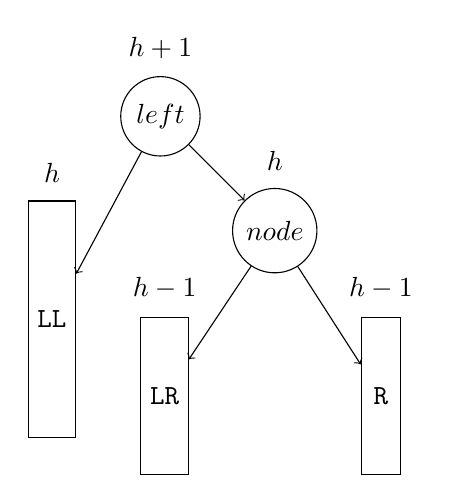
\begin{tikzpicture}
      \node[circle, draw] (left) at (1, 1) {$left$};
      \node[circle, draw] (node) [below right = 1cm of left] {$node$};
      \node[rectangle, minimum height = 3cm, minimum width = 0.5cm, draw] (subtreeLL) [below left = 1cm of left] {\texttt{LL}};
      \node[rectangle, minimum height = 2cm, minimum width = 0.5cm, draw] (subtreeLR) [below left = 1cm of node] {\texttt{LR}};
      \node[rectangle, minimum height = 2cm, minimum width = 0.5cm, draw] (subtreeR) [below right = 1cm of node] {\texttt{R}};


      % alturas
      \node [above = 0.1cm of node] {$h$};
      \node [above = 0.1cm of left] {$h + 1$};
      \node [above = 0.1cm of subtreeLL] {$h$};
      \node [above = 0.1cm of subtreeLR] {$h - 1$};
      \node [above = 0.1cm of subtreeR] {$h - 1$};

      \draw (left) edge[->] (node);
      \draw (node) edge[->] (subtreeR);
      \draw (left) edge[->] (subtreeLL);
      \draw (node) edge[->] (subtreeLR);
    \end{tikzpicture}
  }
  \caption{Rotação simples à direita.  Nós representados como círculos
    e sub-árvores como retângulos.  Acima dos nós e sub-árvores,
    representamos sua altura.}
\end{figure}

\begin{figure}
  \centering
  \subfigure[Antes da rotação]{
    \scalebox{0.6}{
      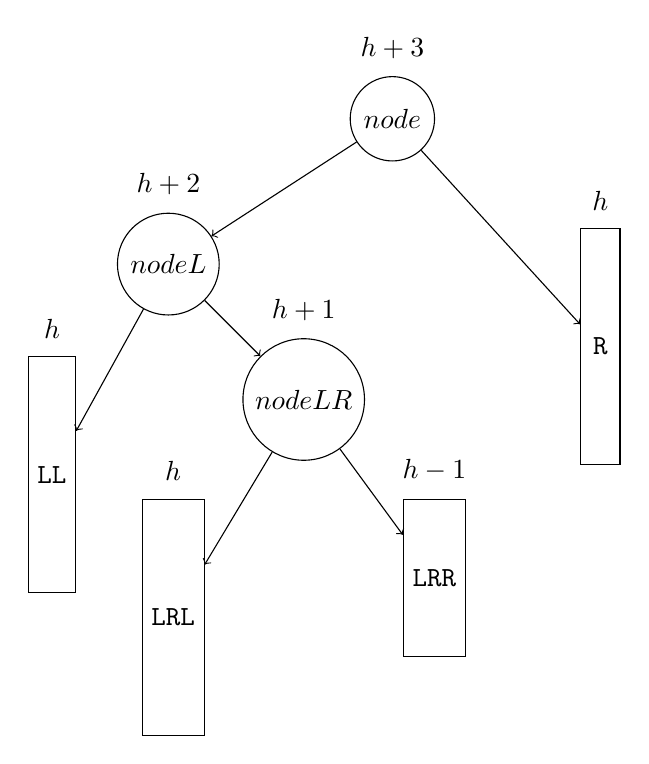
\begin{tikzpicture}
        \node[circle, draw] (node) at (1, 1) {$node$};
        \node[rectangle, minimum height = 3cm, minimum width = 0.5cm, draw] (subtreeR) [below right = 1cm and 2cm of node] {\texttt{R}};
        \node[circle, draw] (nodeL) [below left = 1cm and 2cm of node] {$nodeL$};
        \node[circle, draw] (nodeLR) [below right = 1cm of nodeL] {$nodeLR$};
        \node[rectangle, minimum height = 3cm, minimum width = 0.5cm, draw] (subtreeLL) [below left = 1cm of nodeL] {\texttt{LL}};
        \node[rectangle, minimum height = 3cm, minimum width = 0.5cm, draw] (subtreeLRL) [below left = 1cm of nodeLR] {\texttt{LRL}};
        \node[rectangle, minimum height = 2cm, minimum width = 0.5cm, draw] (subtreeLRR) [below right = 1cm of nodeLR] {\texttt{LRR}};

        \node [above = 0.1cm of subtreeLRL] {$h$};
        \node [above = 0.1cm of subtreeLRR] {$h - 1$};
        \node [above = 0.1cm of nodeLR] {$h + 1$};
        \node [above = 0.1cm of subtreeLL] {$h$};
        \node [above = 0.1cm of nodeL] {$h + 2$};
        \node [above = 0.1cm of subtreeR] {$h$};
        \node [above = 0.1cm of node] {$h + 3$};
        
        \draw (node) edge[->] (subtreeR);
        \draw (node) edge[->] (nodeL);
        \draw (nodeL) edge[->] (subtreeLL);
        \draw (nodeL) edge[->] (nodeLR);
        \draw (nodeLR) edge[->] (subtreeLRL);
        \draw (nodeLR) edge[->] (subtreeLRR);
      \end{tikzpicture}
    }
  }
  \subfigure[Depois da primeira rotação]{
    \scalebox{0.6}{
      \begin{tikzpicture}
        \node[circle, draw] (node) at (1, 1) {$node$};
        \node[rectangle, minimum height = 3cm, minimum width = 0.5cm, draw] (subtreeR) [below right = 1cm and 2cm of node] {\texttt{R}};
        \node[circle, draw] (nodeLR) [below left = 1cm of node] {$nodeLR$};
        \node[circle, draw] (nodeL) [below left = 1cm and 2cm of nodeLR] {$nodeL$};
        \node[rectangle, minimum height = 3cm, minimum width = 0.5cm, draw] (subtreeLL) [below left = 1cm of nodeL] {\texttt{LL}};
        \node[rectangle, minimum height = 3cm, minimum width = 0.5cm, draw] (subtreeLRL) [below right = 1cm of nodeL] {\texttt{LRL}};
        \node[rectangle, minimum height = 2cm, minimum width = 0.5cm, draw] (subtreeLRR) [below right = 1cm of nodeLR] {\texttt{LRR}};

        \node [above = 0.1cm of subtreeLL] {$h$};
        \node [above = 0.1cm of subtreeLRL] {$h$};
        \node [above = 0.1cm of nodeL] {$h + 1$};
        \node [above = 0.1cm of subtreeLRR] {$h - 1$};
        \node [above = 0.1cm of nodeLR] {$h + 2$};
        \node [above = 0.1cm of subtreeR] {$h$};
        \node [above = 0.1cm of node] {$h + 3$};

        \draw (node) edge[->] (subtreeR);
        \draw (node) edge[->] (nodeLR);
        \draw (nodeL) edge[->] (subtreeLL);
        \draw (nodeL) edge[->] (subtreeLRL);
        \draw (nodeLR) edge[->] (subtreeLRR);
        \draw (nodeLR) edge[->] (nodeL);
      \end{tikzpicture}
    }
  }
  \subfigure[Depois da segunda rotação]{
    \scalebox{0.6}{
      \begin{tikzpicture}
        \node[circle, draw] (nodeLR) at (1, 1) {$nodeLR$};
        \node[circle, draw] (nodeL) [below left = 1cm and 2cm of nodeLR] {$nodeL$};
        \node[circle, draw] (node) [below right = 1cm and 2cm of nodeLR] {$node$};
        \node[rectangle, minimum height = 3cm, minimum width = 0.5cm, draw] (subtreeLL) [below left = 1cm of nodeL] {\texttt{LL}};
        \node[rectangle, minimum height = 3cm, minimum width = 0.5cm, draw] (subtreeLRL) [below right = 1cm of nodeL] {\texttt{LRL}};
        \node[rectangle, minimum height = 3cm, minimum width = 0.5cm, draw] (subtreeR) [below right = 1cm and 2cm of node] {\texttt{R}};
        \node[rectangle, minimum height = 2cm, minimum width = 0.5cm, draw] (subtreeLRR) [below left = 1cm of node] {\texttt{LRR}};

        \node [above = 0.1cm of subtreeLL] {$h$};
        \node [above = 0.1cm of subtreeLRL] {$h$};
        \node [above = 0.1cm of subtreeLRR] {$h - 1$};
        \node [above = 0.1cm of subtreeR] {$h$};
        \node [above = 0.1cm of nodeL] {$h + 1$};
        \node [above = 0.1cm of node] {$h + 1$};
        \node [above = 0.1cm of nodeLR] {$h + 2$};

        \draw (nodeLR) edge[->] (node);
        \draw (nodeLR) edge[->] (nodeL);
        \draw (nodeL) edge[->] (subtreeLL);
        \draw (nodeL) edge[->] (subtreeLRL);
        \draw (node) edge[->] (subtreeR);
        \draw (node) edge[->] (subtreeLRR);
      \end{tikzpicture}
    }
  }
  \caption{Rotação dupla: à esquerda em um nível mais baixo, e à
    direita em um nível mais alto.  Nós são círculos e sub-árvores são
    retângulos.}
\end{figure}

\end{document}

%%% Local Variables:
%%% mode: latex
%%% TeX-master: t
%%% End:
